%Always-Imports
\documentclass[12pt, letterpaper]{article}
\usepackage[utf8]{inputenc}
\usepackage[margin=1in]{geometry}

%Sometimes imports
\usepackage{comment}
\usepackage{graphicx}

%biblatex (as opposed to bibtex) parts
%\usepackage[style=numeric]{biblatex}
%\addbibresource{citations.bib}

\begin{comment}
\usepackage{listings} % Typeset Python
\lstset{breaklines=true}
\end{comment}

\title{COSC 5010-03 (23194) Spring 2023 Project Design Document}
\author{Michael Elgin}
\date{April 2, 2023}

\begin{document}

\maketitle

\section{Purpose}

This design document is for a software application that creates secure data files, such as for journaling or otherwise storing private information. The topic this software addresses is privacy concerns when engaging with technology. With cloud services like OneDrive rising in popularity, there are security concerns with respect to the fact that these cloud services are generally not zero-knowledge cloud systems, i.e. the cloud service provider (such as Microsoft) could read the data and/or transfer it to intelligence agencies. This software will create encrypted journal files, and allow them to be read only by the software application while it is used by a user who possesses the correct password, regardless of where the associated files are kept.

\section{Components}
\subsection{GUI}

The GUI will allow the user to interact with the system visually instead of using a command line. It will allow for interacting with files that are encrypted based on the supplied password. In addition it will give the user create-read-update-delete (CRUD) functionality to all accessible files.

\subsection{Password Security Checker}

This component will provide standard checks on a password to ensure it is secure, such as length, use of numbers/capitals/specials/etc. It will warn the user if their chosen password is insecure and allow them to override this if desired by the user.

\subsection{Middleware}

This connects all the components together. It contains the main function that runs at startup, causes the GUI to launch, and everything else to happen. It handles the cryptography, and will most likely base an encryption key off a hash of a user password.

\subsection{Data Files}

These files will be the journal documents which are securely encrypted. At no time will these ever sit at rest on the file system decrypted. They will have their own unique file extension to help identify them on the file system.

\section{Component Interactions}

The middleware will be the starting point of the program; it will launch the GUI and be the only channel of interaction to it. The GUI allows the user to make calls to the middleware through buttons and menus, which in turn interacts with the password security checker and the datafiles. Middleware interacts with the password security checker by importing it. Middleware interacts with datafiles through file system read/write operations.
The GUI, password security checker, and data files have no direct interactions between themselves; they are completely mediated by the middleware.

\section{Security Challenges and Assumptions}

\subsection{Challenges}
The first challenge is privacy design. It must be that the contents of data files are kept secret. If a data file is acquired by anyone other than someone who has the password, it should not be readable. A second challenge is to ensure the passwords created by the user are secure i.e. they do not choose passwords that would be easily guessed, brute-forced, or otherwise learned by an attacker. A third challenge is that the encryption key must be based off the password in a secure way. There should be no shortcuts from the password to the key.

\subsection{Assumptions}
One assumption as per Kerckhoff's principle is that the software itself, including its code, need not be hidden. The same instance of it could securely be used by multiple different users, even in the same working directory, so long as passwords are kept secret. A second assumption is that the cryptography library will also ensure integrity with message authentication codes.

This software is not a distributed system, and the security concerns of a distributed system are not relevant here. However, if a data file were to be sent across a network, it should still be secure by virtue of its encryption.

\section{Addendum April 26, 2023 - 5010 Extension}

\subsection{High-level proof sketch}

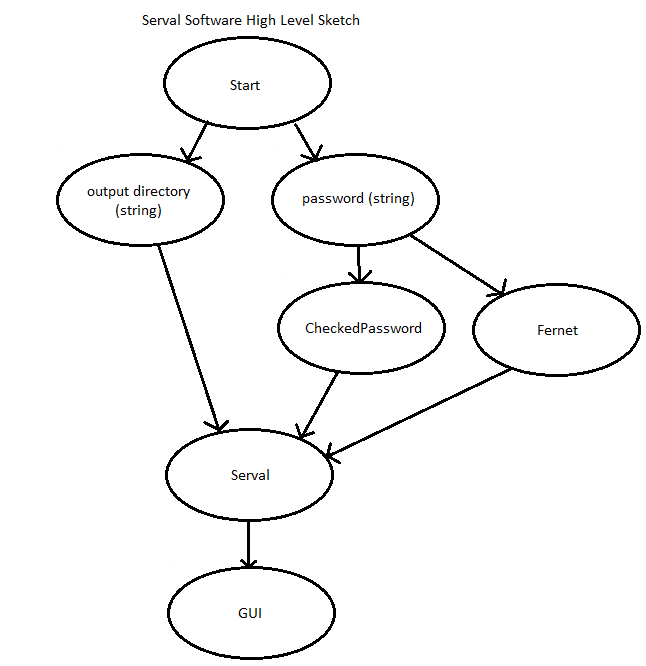
\includegraphics[scale=0.4]{High_Level_Proof_Sketch.png}

\subsection{External threats}

One possible threat from an attacker is to change the contents of a .serval file. Though because of the HMAC built into the fernet tokens, this will be detected and an exception will be thrown. Type checking that the returned contents are not None will prevent such meddling from being passed through the chain of execution.

\subsection{The system being run on}

The software is designed and expected to be portable to any system that can run Python 3.11. As such it makes no mention of any particular operating system or hardware. One threat is that the system may mishandle .serval files. The use of types is meant to ensure that no matter how any underlying system may mishandle the storage of .serval files, the software always receives the proper type to operate on. 

\subsection{Threats created by interfacing}

The most prominent threat created by interfacing is of course the possibility (intentional or not) of an interfacing component passing the wrong type. By using types in functions within the system, the need for input validation is significantly reduced; there need only be checks on the accepted type. Moreover, this also reduces the amount of security vulnerabilities by virtue of there being fewer unhandled exceptions. Another threat is that different versions of dependencies may return different types. To mitigate any differences in types that may be returned by dependency versions, specific versions of dependencies are strictly enforced.

% (when done) Basically look thru all the types in everything everywhere and hypothesize what could go wrong if someone stuck something bad in there. Then explain, along with your types(/typehints) how you're checking to prevent that.

\end{document}